\documentclass{IEEEtran}

\usepackage[utf8]{inputenc} % set input encoding (not needed with XeLaTeX)
\usepackage{geometry}
\geometry{letterpaper}
%%% Examples of Article customizations
% These packages are optional, depending whether you want the features they provide.
% See the LaTeX Companion or other references for full information.



\usepackage{graphicx} % support the \includegraphics command and options

% \usepackage[parfill]{parskip} % Activate to begin paragraphs with an empty line rather than an indent

%%% PACKAGES
\usepackage{url}
\usepackage{booktabs} % for much better looking tables
\usepackage{array} % for better arrays (eg matrices) in maths
\usepackage{paralist} % very flexible & customisable lists (eg. enumerate/itemize, etc.)
\usepackage{verbatim} % adds environment for commenting out blocks of text & for better verbatim
\usepackage{subfig} % make it possible to include more than one captioned figure/table in a single float
\usepackage{algorithm} 
\usepackage{algorithmic}



% These packages are all incorporated in the memoir class to one degree or another...

%%% HEADERS & FOOTERS
%\usepackage{fancyhdr} % This should be set AFTER setting up the page geometry
%\pagestyle{fancy} % options: empty , plain , fancy
%\renewcommand{\headrulewidth}{0pt} % customise the layout...
%\lhead{}\chead{}\rhead{}
%\lfoot{}\cfoot{\thepage}\rfoot{}

%%% END Article customizations

%%% The "real" document content comes below...

\title{VHash: A Voronoi-Based Multidimensional Distributed Hash Table}
\author{Brendan Benshoof \qquad Andrew Rosen  \\Department of Computer Science, Georgia State University\\  bbenshoof@cs.gsu.edu \qquad rosen@cs.gsu.edu }
\date{} % Activate to display a given date or no date (if empty),
         % otherwise the current date is printed 

\begin{document}
\maketitle

\begin{abstract}
%1. State the problem
Distributed Hash Tables are used as a tool to generate overlay networks for P2P networks. Current DHT techniques are not designed to take the nature of the underlying network into account when organizing the overlay network. Current DHT networks assign nodes locations in a ring or tree, limiting the ability of these networks to be more efficient.
%2. Say why it’s an interesting problem
A DHT technique that allows for efficient construction of an overlay network that takes into account the real underlying network would allow for higher performance and faster P2P networks.
%3. Say what your solution achieves
We present VHash as a spacial DHT based on approximate Delaunay Triangulation to integrate distance information between nodes into overlay network topology.
%4. Say what follows from your solution
VHash allows for the creation of P2P networks with faster record lookup time, storage, and maintenance with a geographically diverse set of nodes.

\end{abstract}
\section{Introduction}
A Distributed Hash Table is used provide an overlay network for many P2P applications. State of the art DHT techniques are built on tree or log-ring structures to ensure that the routing distance is $O(lg(n))$ hops between nodes. These topologies, while sufficient in reasonably local networks, do not take into account the lengths or latencies of routes defined by the topology, assuming that every hop has similar latency and throughput. For a global network, a more intelligent means of generating a dynamic overlay network with efficient routing, storage, and backups is needed for future P2P applications. 

We present VHash as a DHT designed to take inter-node latency information into account when generating an overlay on a massive scale.  VHash creates a

Our paper presents the following:
\begin{itemize}
	\item We define how VHash functions.
	\item We show how file sharing and fault tolerance works.
	\item We do some simulations to prove it works.
	\item We present the related work.
	\item We present our future work.
\end{itemize}

Two difficulties that arise in attempting to use Voronoi Tessellation for constructing a DHT.


\section{VHash}






VHash is generalization of ring-based DHTs like Chord \cite{chord}, Pastry , and Symphony from 1-dimensional keyspaces to keyspaces with any number of dimensions.  


VHash was created to allow for spacial representations to be mapped to hash locations, a feature lacking in many current distributed hash tables.  In particular, we aimed to construct a mechanism for creating a more efficient global scale DHT built on a minimal latency overlay. Rather than focus on minimizing the amount of hops required to travel from point to point we wish to minimize the time required for a message to reach its recipient. VHash actually has a worse worst case hop distance ($O(\sqrt[d]{n})$) than other comparable distributed hash tables ($O(lg(n))$). However, VHash can route messages as quickly as possible rather than traveling over a grand tour that an overlay network may describe in the real world.

The naive method of doing so is to assign coordinates to servers based on the geographic location of nodes. More complex approaches would approximate a minimum latency space based on inter-node latency. VHash can be considered  a generalized extension of VoroNet \cite{voronet}. 
%Why is Voronet not okay and why is VHash
Algorithm \ref{latency} describes the process for performing a minimum latency embedding using VHash.

%The intent is that meaning can be ascribed to locations in the DHT and facilitate more efficent function. 
%Specifically in this example we seek to build a minimal latency overlay network for the DHT so a global scale DHT is viable and efficent. 

Chord, if it were generalized out to $d$ dimensions without finger tables would have a lookup time of $\sqrt[d]{n}$.





\begin{itemize}
	\item Assignment of keys and responsibility.  IN Chord it is the successor, Pastry is closest to id.
	\item Pastry's locality heuristic assumes Euclidean space, namely triangle equality holds.  How do we get around that.   Pastry also assumes magic distance function is provided to determine distance between two nodes, however distance is not embedded in the keyspace (which is randomly distributed) but rather the ``proximity space''  built off of bootstrapped assumetions (node we are using to joining the ring is close to the joining node in the proximity space, and the proximity assumptions for a network were good prior to the join operation.  The key idea is that at each hop messages travel closer to the destination, while minimizing the metric distance traveled  (such as num hops).  Expected distance traveled grows exponentially with each hop.  their results showed that the metric distance traveled by routed message over pastry was 30\%-40\% greater than the distance between the source and destination.  Has to uyse second stage when joining to maintain locality.  Total join cost in messages is $\approx 3 \cdot 2^b \cdot \log_{2^{b}} N $
	\item Cost of computing the Voronoi region.  We get around this by accurately approximating it and letting our fault tolerance mechanisms handle any discrepancies until the network repairs itself.
\end{itemize}








\begin{algorithm}
\caption{VHash Minimum Latency Embedding}
\label{latency}
\begin{algorithmic}[1]  % the number is how many 
	\STATE $d$ is the dimensions of the hash space
    \STATE seed the space with $d+1$ nodes at random locations
   	\STATE A node $n$ wishes to join the network
    \STATE $n$ pings a random subset of peers to find latencies $L$
    \STATE Normalize $L$ onto (0.0,1.0) to yield $L_N$
    \STATE Choose position $p$ that minimizes $$\sum\limits_{i\in peers}(L_N[i]-dist(p,i))^2$$ 
    \STATE Re-evaluate location periodically
\end{algorithmic}
\end{algorithm}





\subsection{Key Generation - Mapping a Node to Coordinates}

We suggest using the following spaces as our dimensions

\subsubsection{Cryptographic Keyspace}

\subsubsection{Latency - Spring Based Model}

\subsubsection{Security/Trust Space}

\subsection{Node Degree}

\subsubsection{Average Case}
Avg. Node degree is the average degree of a point in a $d$-dimensional toroidal space.  
Consider a $d$-dimensional toroidal space.  Let some arbitrary point $A$ be the center of this space\footnote{Any point in a toroidal space can view itself as it's center}.  A hypercube that surrounds the space would be defined by $3^d -1$ points citation \footnote{Is this rigorous enough?}

\subsubsection{Worst Case}


The expected maximum degree of a ?point?  in $d$-dimensional Delaunay Triangulation is $\Theta(\frac{\log n}{\log \log n} )$ \cite{bern1991expected}.  We don't know how this is effected by toroidal spaces.



\subsection{Memory Overhead}
In order to route, a node maintains a routing table consisting of the nodes it borders a region with.  Unlike other DHTs, which keep routing tables of a set size, VHash's routing table depends on the nodes that it shares a border with, which is on average $3^d -1$


 
\subsection{Toroidal Distance Equation}

Given two vector locations $\vec{a}$ and $\vec{b}$ on a  $d$ dimensional unit toroidal hypercube:
\[ distance = \sqrt[|d|]{\sum\limits_{i\in d} (\min(|\vec{a}_i-\vec{b}_i|,1.0-|\vec{a}_i-\vec{b}_i|))^2}\]

\subsection{Mechanism}
VHash maps nodes to a $d$ dimension toroidal unit space overlay. This is essentially a hypercube with wrapping edges. The toroidal property makes visualization difficult but allows for a space without a sparse edge, as all nodes can translate the space such that they are at the center of the space.  In effect, each node views itself at the center of the graph.

VHash nodes are responsible for the address space defined by their Voronoi region. This region is defined by a list of peer nodes maintained by the node. A minimum list of peers is maintained such that the node's Voronoi region is well defined. The links connecting the node to its peers correspond to the links of a Delaunay Triangulation.  One such possible network is shown on Figure \ref{churninit}.


\begin{figure}
    %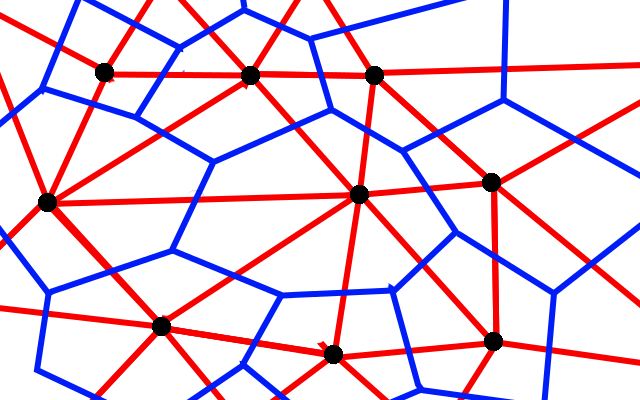
\includegraphics[width=\linewidth]{voronoi-churn2}
    \caption{The starting network topology.  The blue lines demark the Voronoi edges, while the red lines connecting the nodes correspond to the Delaunay Triangulation edges and one-hop connections.}
    \label{churninit}
\end{figure}

\subsection{Relation to Voronoi Diagrams and Delaunay Triangulation}

VHash does not strictly solve Voronoi diagrams \cite{voronoi}, as the toroidal nature of the space preclude the traditional means of solving for Voronoi regions. However, VHash's peer management approximates a topology with similar properties. 
%Rather than attempt to calculate the Voronoi region of each node, it simply filters locations, assigning responsibility to the nearest node. 
An online algorithm (Algorithm \ref{peer} maintains the set of peers defining the node's Voronoi region. The set of peers required to define a node's Voronoi Region corresponds to a solution to the dual Delaunay Triangulation.



\begin{algorithm}
\caption{VHash Greedy Peer Selection}
\label{peer}
\begin{algorithmic}[1]  % the number is how many 
	\STATE $Candiates$ is the set of candidate peers
    \STATE $Peers$ is the set of this node's peers
    \STATE $Canidates$ is sorted by each node's closeness to this node
    \STATE The closest member of $Canidates$ is popped and added to $Peers$
    \FORALL{$n$ in $Canidates$}
    	\STATE $c$ is the midpoint between this node and $n$
        \IF{Any node in $Peers$ is closer to $c$ than this node}
        	\STATE reject $n$ as a peer
        \ELSE
        	\STATE Add $n$ to $Peers$
        \ENDIF
    \ENDFOR
\end{algorithmic}
\end{algorithm}


\subsection{Messages}
Maintenance and joining are handled by a simple periodic mechanism. A notification message consisting of a node's information and active peers is the only maintenance message. All messages have a destination hash location which is used to route them to the proper server. This destination can be the hash location of a particular node or the location of a desired record or service.  The message is received by the node responsible for the location. Services running on the DHT define their own message contents, such as commands to store and retrieve data.

\subsection{Message Routing}
Messages are routed over the overlay network using a simple algorithm ( Algorithm \ref{routing}). 
When routing a message to an arbitrary location, a node calculates who's Voronoi region the message's destination is in amongst the itself and its peers. If the destination falls within its own region, then it is responsible and handles the message accordingly. Otherwise, the node forwards the message to the closest peer to the destination location. This process describes\footnote{Wording.  Is equivalent a better word?} a pre-computed and cached A* routing  algorithm \cite{astar} . 

\begin{algorithm}
\caption{Vhash Routing}
\label{routing}
\begin{algorithmic}[1]  % the number is how many 
	\STATE $P_0$ is this node's set of peers
    \STATE $N$ is this node
	\STATE $m$ is a message addressed for $L$
    \STATE $Forwards$ is the set $P_0\cup{}N$
    \STATE find $C$: member of $Forwards$ which has the shortest distance to $L$
    \IF{$C$ is $N$}
    	\STATE $N$ is the responsible party.
        \STATE Handle $m$
    \ELSE
    	\STATE Forward $m$ to $C$ for handling or further routing
    \ENDIF
\end{algorithmic}
\end{algorithm}

\subsection{Joining and Maintenance}
Joining the network is a straightforward process. A new node first learns the location of at least one member of the network to join. The joining node then choses a location in the hash space either at random or based on a problem formulation (for example, based on geographic location or latency information).

After choosing a location, the joining node sends a "join" message to its own location via the known node.
The message is forwarded to the current owner of that location who can be considered the "parent" node.
The parent node immediately replies with a maintenance message containing its full peer list. This message is sent to the joining node, who then uses this to begin defining the space it is responsible for. 

The joining node's initial peers are a subset of the parent and the parent's peers. The parent adds the new node to its own peer list and removes all his peers occluded by the new node.  Then regular maintenance propagates the new node's information and repairs the overlay topology.  This process is described by Algorithm \ref{join}.

\subsection{Eclipse and Sybil Attacks}

\begin{algorithm}
\caption{Vhash Join}
\label{join}
\begin{algorithmic}[1]  % the number is how many 
\STATE new node $N$ wishes to join and has location $L$
\STATE $N$ knows node $x$ to be a member of the network
\STATE $N$ sends a request to join, addressed to $L$ via $x$
\STATE node $Parent$ is responsible for location $L$ and receives the join message
\STATE $Parent$ sends to $N$ its own location and list of peers
\STATE $Parent$ integrates $N$ into its peer set
\STATE $N$ builds its peer list from $N$ and its peers
\STATE regular maintenance updates other peers
\end{algorithmic}
\end{algorithm}


Each node in the network performs maintenance periodically by a maintenance message to its peers. The maintenance message consists of the node's information and the information on that node's peer list. When a maintenance message is received, the receiving node considers the listed nodes as candidates for its own peer list and removes any occluded nodes (Algorithm \ref{peer}). 

When messages sent to a peer fail, it is assumed the peer has left the network. The leaving peer is removed from the peer list and candidates from the set of 2-hop peers provided by other peers move in to replace it.  Maintenance is described by Algorithms \ref{maint} and \ref{handlemaint}.  Figures \ref{churnjoin}, \ref{churndone}, and \ref{churndrop} illustrate the joining processing.

\begin{algorithm}
\caption{VHash Maintenance Cycle}
\label{maint}
\begin{algorithmic}[1]  % the number is how many 
	\STATE $P_0$ is this node's set of peers
    \STATE $T$ is the maintenance period
    \WHILE{Node is running}
    	\FORALL{node $n$ in $P_0$}
        	\STATE Send a Maintenance Message containing $P_0$ to $n$
        \ENDFOR
    \STATE Wait $T$ seconds
    \ENDWHILE
\end{algorithmic}
\end{algorithm}


\begin{algorithm}
\caption{VHash Handle Maintenance Message}
\label{handlemaint}
\begin{algorithmic}[1]  % the number is how many 
	\STATE $P_0$ is this node's set of peers
	\STATE Receive a Maintenance Message from peer $n$ containing its set of peers:$P_n$
    \FORALL{Peers $p$ in $P_n$}
    	\STATE Consider $p$ as a member of $P_0$
        \IF{$p$ should join $P_0$}
        	\STATE Add $p$ to $P_0$
            \FORALL {Other peers $i$ in $p$}
            	\IF{$i$ is occluded by $p$}
                	\STATE remove $i$ from $P_0$
                \ENDIF
            \ENDFOR
        \ENDIF
    \ENDFOR
\end{algorithmic}
\end{algorithm}

There is no function for a "polite" exit from the network. VHash  assumes nodes will fail and the difference between an intended failure and unintended failure is unnecessary. The only issue this causes is that node software should be designed to fail totally when issues arise rather then attempt to fulfill only part of its responsibilities.  


\begin{figure}
    %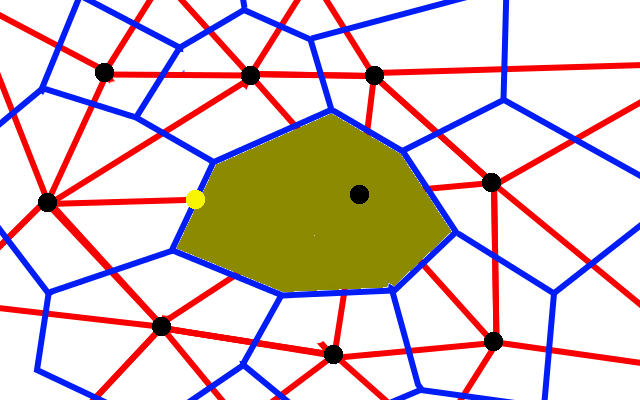
\includegraphics[width=\linewidth]{voronoi-churn4}
    \caption{Here, a new node is joining the networks and has established that his position falls in the the yellow shaded Voronoi region.}
\end{figure}


\begin{figure}
    %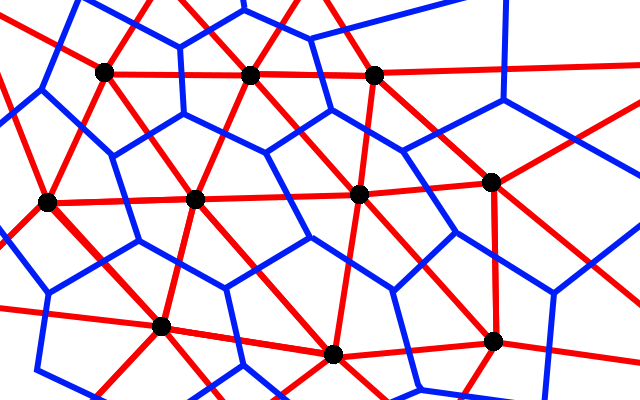
\includegraphics[width=\linewidth]{voronoi-example}
    \caption{The network topology after the new node has finished joining.}
    \label{churndone}
\end{figure}

\begin{figure}
    %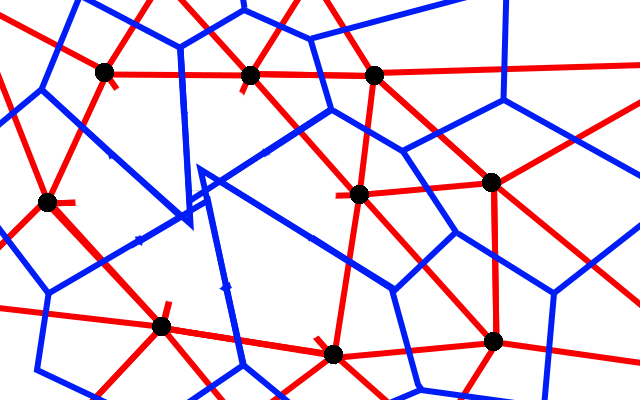
\includegraphics[width=\linewidth]{voronoi-churn1}
    \caption{The topology immediately after the new node leaves the network. After maintenance takes place, the topology repairs itself back to the configuration shown in Figure \ref{churninit}.}
    \label{churndrop}
\end{figure}


\subsection{Data Storage and Backups}
The primary goal of a DHT is to provide a distributed storage medium. We extend this idea to distribute work and information among nodes using the same paradigm. Resources in the network, be it raw data or assigned tasks, are assigned hash locations. The node responsible for a given hash location is responsible for the maintenance of that resource. When a node fails, its peers take responsibility of its space. Thus it is important to provide peers with frequent backups of a node's assigned resources.  That way, when a node fails, its peers can immediately assume its responsibilities.

When a resource is to be stored on the network, it is assigned a hash location. The hash locations assigned could be random, a hash of an identifier, or have specific meaning for an embedding problem. The node responsible for that resource's hash location stores the resource.

A resource is accessed by contacting the node responsible for the resource.  However, the requester generally has no idea which node is responsible for any particular resource.  The data request messsage is addressed to the location corresponding to the resource, rather than the node responsible for that location.  The message is forwarded over the overlay network, each hop bringing the node closer until it reaches the responsible node, who sends the resource or an error if the resource does not exist.

Some options are immediately apparent for dealing with wasted storage space. A system that is primarily read driven can record the time of the last read or a frequency of reads such that resources that are not read often enough are deleted after a certain period of time. If a system is write driven, allow the resource to be assigned a time to live, which can be updated as needed.

A node periodically sends a message containing backups of the resources for which it became newly responsible for to each of its peers. To minimize bandwidth and time wasted by backups, the node should only send the records changed since last backup.

\section{Related Work}
Voronet stuff here.


\section{Conclusions and Future Work}
Apply this to MANET.


\bibliographystyle{ieeetr}
\bibliography{P3DNS}
\end{document}
